% This is samplepaper.tex, a sample paper demonstrating the
% LLNCS class package for the SMU Data Science Review Journal;
%
% This sample paper is a modified version of samplepaper.tex for
% the Springer Computer Science proceedings; Version 2.20 of 2017/10/04
%
% Version 1.0 2019/06/03

% Use the llncs.cls formatting
\documentclass{llncs}

% Set the packages for use within the document. The following
% packages should be included.  Additional packages that do not
% conflict with these packages or change the llncs class formatting
% may be used.  Packages that do change the formatting are
% not allowed.
\usepackage{graphicx} % Used for displaying a sample figure.
% If possible, figure files should be included in EPS format.
% PDF format is also acceptable. JPEG  will work, but some of
% them are downsampled resulting in fuzzy images.
\usepackage{booktabs} % Better horizontal rules in tables
\usepackage{multirow} % Better combined rows in tables

% The title of the paper
\title{Sample Title for a Paper Published in the SMU Data Science Review Journal}

% The complete list of authors with their affiliations
\author{
First Author\inst{1} \and
Second Author\inst{1,2,3} \and
Third Author\inst{3}
}

% The Institutes and emails associated with each author. All students
% should use their MSDS affiliation or a generic SMU affiliation.
% Advisors should use their appropriate affiliation. Note that advisors
% are NOT referenced or otherwise denoted as advisors. Advisors
% are simply co-authors on the paper.
% Note that the emails for the MSDS affiliation, show how
% to list emails that have the same organization portion.
\institute{
Master of Science in Data Science, Southern Methodist University,
Dallas TX 75275 USA
\email{\{fauthor,sauthor\}@smu.edu} \and
Springer Heidelberg, Tiergartenstr. 17, 69121 Heidelberg, Germany
\email{lncs@springer.com} \\
\url{http://www.springer.com/gp/computer-science/lncs} \and
ABC Institute, Rupert-Karls-University Heidelberg, Heidelberg, Germany\\
\email{\{abc,lncs\}@uni-heidelberg.de}
}

% Begin the document
\begin{document}

\maketitle              % typeset the title and author of the paper

% Reset the footnote counter
\setcounter{footnote}{0}
% The abstract environment uses the \begin{} and \end{} constructs to
% denote the beginning and ending of the abstract contents.
\begin{abstract}
The abstract should briefly summarize the contents of the paper in
150--250 words.  The abstract should contain approximately six sentences contained within a single paragraph. The first sentence typically begins with ``In this paper, we present'' which is then followed by what is presented in the paper.  The second sentence is used to motivate the importance of what is presented and define the broad problem domain. Then, two to three sentences are used to state how the problem was solved. A single statement of the main result (singular) is then followed by a single statement of the main conclusion (singular).

% Keywords may be used, but they are not required.
%\keywords{First keyword  \and Second keyword \and Another keyword.}
\end{abstract}

% Sections are denoted by the use of the \section{Section Name}
% command -- where "Section Name" is the name you give to the Section.
\section{Introduction}

Your first section should be your {\em Introduction} section. The Introduction is a 3--4 page executive summary of your paper.

% Note that paragraphs are created by placing a blank line before the
% paragraph within the .tex file just as a blank line exists before the
% beginning of this comment. That blank line tells LaTeX to treat the
% following text as a new paragraph.  No other commands are needed.
The Introduction follows the same general organization as the Abstract.

The Introduction should have approximately 8--10 paragraphs.  The first paragraph is ``Motivation'' that states the broad problem and provides details as to why the problem is important. The second paragraph begins with the one sentence problem statement and then has 3--4 sentences adding details as needed.  There should then be 3--4 paragraphs detailing the final approach used to solve the problem.  Then a one paragraph summary of the main results followed by a one paragraph summary of the main conclusions.  The last paragraph should contain an overview of the remainder of the paper organization.

The Introduction section should {\bf NOT} contain tables, figures, or subsections.  This is a simple executive summary.

% A second section is begun with another \section{} command
\section{A Second Section}

% Subsections may be created with a \subsection{} command
\subsection{A Subsection Sample}

Please note that the first paragraph of a section or subsection is
not indented. The first paragraph that follows a table, figure,
equation etc. does not need an indent, either.

Subsequent paragraphs, however, are indented.

%\subsubsection{Sample Heading (Third Level)} Only two levels of headings should be numbered. Lower level headings remain unnumbered; they are formatted as run-in headings.

%\paragraph{Sample Heading (Fourth Level)} The contribution should contain no more than four levels of headings.

Table~\ref{tab1} gives a summary of all heading levels. There should be zero reason to have either a 3rd-level heading or a 4th-level heading. If you feel the need to have such headings, then you should restructure your document such that no 3rd-level or 4th-level headings are needed.

\begin{table}
\caption{Table captions should be placed above the
tables.}\label{tab1}
\begin{center}
\begin{tabular}{ l l l }
\toprule
Heading level &  Example & Font size and style\\
\midrule
Title (centered) &  {\Large\bfseries Lecture Notes} & 14 point, bold\\
1st-level heading &  {\large\bfseries 1 Introduction} & 12 point, bold\\
2nd-level heading & {\bfseries 2.1 Printing Area} & 10 point, bold\\
3rd-level heading & {\bfseries Run-in Heading in Bold.} Text follows & 10 point, bold\\
4th-level heading & {\itshape Lowest Level Heading.} Text follows & 10 point, italic\\
\bottomrule
\end{tabular}
\end{center}
\end{table}


% While you should not need it, if a time comes when you need
% to force the beginning of a paragraph to not be indented, you
% may use the \noindent command.

Displayed and numbered equations such as Equation~\ref{eq:simpleEquation} are centered and set on a separate line.
\begin{equation}
\label{eq:simpleEquation}
x + y = z
\end{equation}

Please try to avoid rasterized images for line-art diagrams and
schemas. Whenever possible, use vector graphics instead (see
Fig.~\ref{fig1}).

\begin{figure}
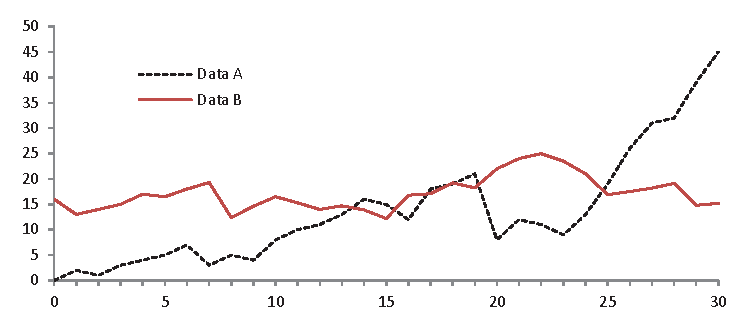
\includegraphics[width=\textwidth]{fig1.eps}
\caption{A figure caption is always placed below the illustration.
Please note that short captions are centered, while long ones are
justified by the macro package automatically.} \label{fig1}
\end{figure}

\begin{theorem}
This is a sample theorem. The run-in heading is set in bold, while
the following text appears in italics. Definitions, lemmas,
propositions, and corollaries are styled the same way.
\end{theorem}
%
% the environments 'definition', 'lemma', 'proposition', 'corollary',
% 'remark', and 'example' are defined in the LLNCS documentclass as well.
%
\begin{proof}
Proofs, examples, and remarks have the initial word in italics,
while the following text appears in normal font.
\end{proof}

For citations of references, we prefer the use of square brackets
and consecutive numbers where the references are numbered according to the ascending alphabet (i.e.,~a to z) of the first author's last name. Citations using labels or the author/year convention are not acceptable. The following reference provides
a sample reference list with entries for journal
articles~\cite{article1,article2}, a chapter~\cite{inbook}, a
book~\cite{book}, and a conference proceedings without editors~\cite{conference}.
 Multiple citations are grouped
\cite{article1,article2,inbook,book,conference}.

Note that URLs should be placed in Footnotes\footnote{More information may be found at \url{http://www.smu.edu}. Last accessed 31 Dec 2018.} and not in the references.  Only documents that will not change over time should be placed in the references and cited.
%
% ---- Bibliography ----
%
% BibTeX users should specify bibliography style 'splncs04'.
% References will then be sorted according to alphabetical
% and formatted in the correct style.
%
 \bibliographystyle{splncs04}
 \bibliography{samplebib}

% End the document
\end{document}
